\chapter{Zestawienie modelowania procesów biznesowych ze specyfiką aplikacji mobilnych}
\label{cha:bpmVSMobileApplications}

Tematem niniejszej pracy magisterskiej jest analiza możliwości adaptacji środowisk uruchomieniowych dla logiki biznesowej na platformach mobilnych. Temat jest szeroki, zarówno środowiska uruchomieniowe dla logiki biznesowej jak i platformy mobilne mogą być rozumiane w różny sposób, dlatego na początku niezbędne jest uściślenie kilku kwestii. Środowiska uruchomieniowe dla logiki biznesowej w niniejszej pracy magisterskiej rozumiane będą przez technologię Modelowania Procesów Biznesowych. W przypadku platform mobilnych największa uwaga zostanie poświęcona najbardziej popularnej, opartej na systemie operacyjnym \textit{Unix} platformie mobilnej - \textit{Android}. Aby przejść do zestawienia tych dwóch technologii niezbędne jest ich poznanie i zrozumienie, dlatego w kolejnych sekcjach niniejszego rozdziału zostaną opisane wyżej wymienione technologie.


%---------------------------------------------------------------------------
\section{Modelowania Procesów Biznesowych}
\label{sec:analizaModelowaniaProcesowBiznesowych}

Modelowanie Procesów Biznesowych jest pojęciem bardzo ogólnym, nie zawiera w sobie żadnych szczegółów technicznych, określa jedynie pewne specyficzne podejście do rozwiązywania problemów informatycznych. W podejściu tym podczas analizy, główny nacisk kładziony jest na wyłonienie procesów występujących w analizowanym problemie. Proces jest tutaj rozumiany jako zbiór następujących w określonej kolejności operacji, prowadzących do osiągnięcia konkretnego celu. Najczęściej modelowanie procesów biznesowych jest rozważane w kontekście działania konkretnego przedsiębiorstwa, w którym wyłonienie procesów oraz odpowiednie nimi zarządzenie ma kluczowe znaczenie dla osiągnięcia sukcesu. 

\subsection{BPM}
\label{sec:bpm}

W literaturze pojęcie modelowania oraz zarządzanie procesami biznesowymi w kontekście przedsiębiorstw występuje pod skrótem BPM, którego angielskie rozwinięcie to \textit{Buisness Process Management} (pl.  Zarządzanie Procesami Biznesowymi). Idea BPM jest bardzo popularna i szeroko rozwijana w środowisku IT, powstała nawet organizacja pod nazwą \textit{European Association of Buisness Process Managment} zajmująca się rozwojem i promocją BPM.  Na stronie internetowej organizacji znaleźć możemy oficjalną definicje BPM, która mówi, że w skład Zarządzania Procesami Biznesowymi wychodzi:
\begin{itemize}
\item projektowanie,
\item wykonywanie,
\item dokumentacja,
\item pomiar,
\item monitorowanie,
\item kontrola
\end{itemize}
zautomatyzowanych oraz niezautomatyzowanych procesów biznesowych~\cite{EAOBPMWeb}.

W środowisku IT zdarza się, że BPM traktowany jest jako osobna klasa systemów informatycznych, obok ERP, MES, CRM itd. Z punktu widzenia przedstawionej wyżej definicji trudno zgodzić się z takim podejściem, można jednak zauważyć że BPM de facto może zostać wykorzystany do realizacji każdego z wymienionych rodzajów oprogramowania lub posłużyć jako narzędzie integrujące wyżej wymienione klasy systemów, w celu stworzenia globalnego systemu zarządzania przedsiębiorstwem~\cite{wiBPMA}.

\subsection{Projektowanie procesów biznesowych}
\label{sec:projektowanieBPM}

Zdecydowanie jednym z najistotniejszych etapów w tworzeniu systemu opartego o procesy biznesowe jest etap projektowania. Jednym z najbardziej popularnych narzędzi do tego celu jest BPMN (\textit{Buisness Process Model and Notation}), które doczekało się już dwóch wersji. W kontekście niniejszej pracy magisterskiej notacja BPMN nie jest szczególnie ważna jednak została wspomniana ze względu na jej wykorzystanie w przykładach. BPMN z jednej strony jest narzędziem do graficznego modelowania procesów biznesowych, jest to pewien standard, który z założenia ma być intuicyjny dla osób z poza środowiska IT. Z drugiej zaś strony istnieją narzędzia pozwalające za pomocą BPMN modelować procesy które są bezpośrednio uruchamiane na konkretnych platformach~\cite{BPMN}. 

\begin{figure}[h]
\centerline{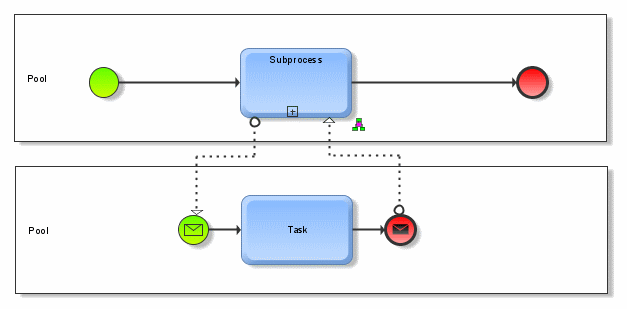
\includegraphics[scale=0.8]{BPMN_example}}
\caption{Przykładowy proces BPMN.}
\label{fig:BPMN_example}
\end{figure}

\subsection{Wykonywanie procesów biznesowych}
\label{sec:wykonywanieBPM}

Jak zostało wspomniane na samym początku Modelowanie Procesów Biznesowych jest pojęciem ogólnym nie wskazującym konkretnej technologii, która ma posłużyć do wykonania procesów biznesowych. Z definicji można jednak wnioskować, że środowiskiem do wykonywania procesów biznesowych w przedsiębiorstwach na pewno nie powinna być prosta aplikacja desktopowa czy mobilna. Biorąc pod uwagę wachlarz zastosowań BPM nie trudno dojść do wniosku, że najbardziej odpowiednim środowiskiem dla procesów biznesowych są środowiska aplikacji rozproszonych. 
Powyższe stwierdzenie potwierdza przegląd istniejących systemów uruchomieniowych dla procesów biznesowych. W ogromnej większości są to aplikacje internetowe. 

\subsection{Podsumowanie}
\label{sec:podsumowanieBPM}

Z punktu widzenia niniejszej pracy magisterskiej, głównym wnioskiem płynącym z powyższego opisu BPM jest skala problemów rozwiązywanych przez to podejście oraz ich usytuowanie w środowisku aplikacji rozproszonych. 

%---------------------------------------------------------------------------
\section{Analiza aplikacji na platformy mobilne}
\label{sec:analizaAplikacjiMobilnych}

Wzrost popularności urządzeń przenośnych takich jak smatrphon czy tablet, wpłynął na powstanie specyficznej klasy systemów informatycznych, zwanych aplikacjami mobilnymi. Aplikacje mobilne cechuje ukierunkowanie na rozwiązywanie wąskiego rodzaju problemów przy pomocy urządzenia dostępnego dla użytkownika niemal 24h na dobę. Szczególną popularność zyskały aplikacje mobilne ukierunkowane na rynek globalny tzn. dla użytkownika masowego. Coraz większą popularność zyskują również aplikacje biznesowe ukierunkowane np. na wymianę danych pomiędzy pracownikami przedsiębiorstwa w celu rozwiązania konkretnego zadania. 

\subsection{Rodzaje aplikacji mobilnych}
\label{sec:rodzajeAplikacjiMobilnych}

Ze względu na rodzaj zastosowania aplikacje mobilne można sklasyfikować w następujący sposób:

\begin{itemize}
\item Samodzielne aplikacje -- aplikacje wykorzystujące tylko i wyłącznie lokalne zasoby urządzenia, korzystające z lokalnej bazy danych bez połączenia z systemami zewnętrznym, często nie wymagające połączenie do internetu. Dobrym przykładem takiej aplikacji może być prosty notatnik.  
\item Aplikacje klienckie -- są to aplikacje bazujące na komunikacji z systemami zewnętrznymi przy pomocy jakiegokolwiek interfejsu komunikacyjnego,  najczęściej połączenia HTTP. Zazwyczaj aplikacje te wykorzystują również lokalną bazę danych umożliwiając użytkownikom pracę z aplikacją w przypadku braku połączenia z systemem zewnętrznym.
\item Internetowe -- najczęściej strony www, aplikacje  te nie wykorzystują lokalnych zasobów urządzeń mobilnych, ich rolą jest udostępnienie prostego interfejsu użytkownika systemu dla użytkowników aplikacji mobilnych.
\item Gry  -- szczególny przypadek samodzielnych aplikacji ukierunkowanych głównie na wykorzystanie lokalnych zasobów urządzenie w celach rozrywkowych, szczególnie eksploatowana w tego typu aplikacjach jest karta graficzna urządzenia.
\end{itemize}

\subsection{Tryby online/offline}
\label{sec:trybyAplikacjiMobilnych}

Najbardziej docenianym rodzajem aplikacji mobilnych z punktu widzenia biznesu są aplikacje klienckie. W przypadku tych aplikacji bardzo istotny jest problem połączenia z systemami zewnętrznymi. Wyróżniamy tutaj dwa tryby pracy aplikacji:

\begin{itemize}
\item Tryb online -- urządzenie udostępnia przynajmniej jeden typ komunikacji bezprzewodowej (Wi-fi, Bluetooth, łącza podczerwieni (IrDa), GPRS). W trybie online aplikacje mobilne mają bezpośredni dostęp do zewnętrznych i zdalnych źródeł danych, innych urządzeń mobilnych lub stacjonarnych systemów komputerowych.   
\item Tryb offline -- urządzenie ma bezpośredni dostęp tylko do lokalnie przechowywanych informacji. Dane te mogą być jednak synchronizowane z innymi urządzeniami w czasie krótkich sesji komunikacyjnych. Wymiana danych podczas synchronizacji może następować w obu kierunkach. 
\end{itemize}

\subsection{Cechy specyficzne dla aplikacji mobilnych }
\label{sec:cechyAplikacjiMobilnych}

Opisując aplikacje mobilnie nie można zapomnieć o cechach specyficznych, które są niezwykle ważne z punktu widzenia projektanta i programisty aplikacji mobilnych. To właśnie dzięki tym cechom aplikacje mobilne posiadają tę, a nie inną specyfikę:

\begin{itemize}
\item Ograniczone zasoby sprzętowe -- urządzenie przenośnie pod względem zasobów sprzętowych nigdy nie zastąpią komputerów stacjonarnych, a tym bardziej urządzeń serwerowych. Właśnie ze względu na tę cechę aplikacje mobilne ukierunkowane są na rozwiązywanie małych - jednostkowych problemów. Projektant aplikacji mobilnych powinien szczególnie zwrócić uwagę na ten aspekt w przypadku projektowania interfejsu do komunikacji z systemami zewnętrznymi. Asplikacje mobilne powinny wykorzystywać lekkie interfejsy komunikacyjne np. REST, aby jak najmniej obciążać kartę sieciową urządzenia. 
\item Uproszczony interfejs użytkownika dostosowany do ekranów dotykowych -- cecha ta jest bardzo ważna głównie dla projektantów graficznych, ale ma również znaczący wpływ na rodzaj zadań rozwiązywanych za pomocą aplikacji mobilnych.  
\item Przerwy w działaniu aplikacji -- aplikacje mobilne w przeciwieństwie do innych rodzajów systemów są szczególnie narażone na przerwy w działaniu. Najprostszym przykładem może być rozmowa telefoniczna przychodząca w trakcie pracy z aplikacją. Najczęściej w takich przypadkach aplikacje przechodzą w tryb uśpienia i nie ma pewności czy praca zostanie wznowiona. Programiści powinny pamiętać o zapamiętywaniu poszczególnych stanów aplikacji aby użytkownik nie tracił wykonanej pracy. 
\item Dostęp do geolokalizacji -- aplikacje mobilne oprócz ograniczeń posiadają również wiele cech dodatkowych, wyróżniających je wśród innych systemów - jedną z nich jest dostęp do  geolokalizacji.  Funkcjonalność ta bardzo szeroko wykorzystywana jest przez systemy zwane \textit{Context Aware Middleware}~\cite{ContextAwareMobility}. 
\item Dostęp do aparatu/kamery -- jest to kolejna cecha rozszerzająca możliwości aplikacji mobilnych, może być wykorzystana na przykład jako narzędzie do skanowania kodów kreskowych, albo sposób dokumentacji pracy wykonanej przez użytkownika systemów mobilnych. 
\item Specyficzna architektura dla różnych systemów operacyjnych -- przyglądając się najbardziej popularnym platformą mobilnym można odnaleźć bardzo wiele cech współnych, mimo wszystko platformy te korzystają zazwyczaj z różnych technologii do realizacji podobnych celów.
\end{itemize}

\subsection{Komunikaty Push}
\label{sec:push}

Ze względu na zmienne warunki w dostępie do mediów komunikacyjnych, aplikacji mobilne wykorzystują w głównej mierze komunikacje typu pull (pobieranie informacji na żądanie) do wymiany informacji z systemami zewnętrznymi. Najpopularniejsze platformy mobilne jak \textit{Android}, \textit{iOS} oraz \textit{Windows Phone} udostępniają również alternatywny sposób komunikacji - push. 

Komunikacja push odbywa się jednak zawsze za pośrednictwem serwisów udostępnianych przez platformy mobilne do tego celu. Komunikacja ta posiada wiele ograniczeń, a już na pewno najważniejszym z nich jest brak pewności, że komunikat zostanie dostarczony. Komunikacja push powinna być zatem wykorzystywana jedynie do notyfikacji użytkownika o jakimś zdarzeniu, a nie do przesyłania informacji kluczowych dla działania aplikacji. 


%---------------------------------------------------------------------------
\section{BPEL „inteligentne” narzędzie integracyjne}
\label{sec:bpel}

BPEL (\textit{Business Process Execution Language}), a właściwie pełna nazwa WS-BPEL,  której rozwinięcie to \textit{Web Services Business Process Execution Language} jest językiem opartym o składnię xml, służącym do wykonywania procesów biznesowych w środowisku usług sieciowych. Język BPEL jest ustandaryzowany przez oranizacje OASIS (\textit{Organization for the Advancement of Structured Information Standards}). 

Organizacja OASIS definiuje język BPEL jako: \textit{Umożliwiający użytkownikom opis aktywności procesów biznesowych jako usługi sieciowe oraz definicję w jaki sposób usługi te mogę być połączone między sobą w celu wykonania zadania}~\cite{OASISweb}.

Jak argumentuje OASIS, język BPEL powstał z konieczności stworzenia dodatkowej warstwy integracyjnej, która wykorzysta potencjał dostarczony przez usługi sieciowe oraz procesy biznesowe. Warto tutaj wspomnieć o historii powstania BPEL. Microsoft i IBM dostrzegając potrzebę stworzenia technologii pozwalającej definiować przepływ wywołań usług sieciowych stworzyli osobne, ale bardzo podobne języki nazwane WSFL (\textit{Web Service Flow Language}) oraz Xlang. W miare wzrostu popularności BPM zdecydowali się połączyć siły aby stworzyć wspólny standard, opisanych za pomocą WSDL. Zarówno Microsoft jak i IBM dostrzegli, że architektura SOA (\textit{Service Oriented Architecture}) wymaga wprowadzenia technologi, która pozwoli składać klocki jakimi są usługi sieciowe w jedną zgrabną całość.

Dotychczasowy model komunikacji udostępniany przez usługi sieciowe był niewystarczający, głównie z powodu braku zachowania stanu podczas prostej komunikacji żądanie-odpowiedź.  Komunikacja ponadto była głównie jednokierunkowa. Model komunikacji dla biznesu wymagał natomiast sekwencyjnej wymiany wiadomości pomiędzy wieloma węzłami. Operacje wykonywane na węzłach mogły trwać bardzo długo, dlatego zainstaniała konieczność obsługi tego typu sytuacji przy pomocy asynchronicznego wywoływania serwisów~\cite{OASISBPELSpec}.

\subsection{Cechy języka BPEL}
\label{sec:bpelFeatures}

\begin{itemize}
\item Definiowane procesy biznesowe komunikują się z usługami sieciowymi przy pomocy WSDL 1.1 i same są usługami sieciowymi opisanymi przez WSDL 1.1.  
\item Do komunikacji pomiędzy usługami wykorzystywany jest protokół SOAP.
\item Procesy zdefiniowane są w języku bazującym na xml.
\item BPEL dostarcza funkcji do wykonywania prostych manipulacji na danych.
\item Posiada wsparcie do identyfikowania instancji procesów.
\item Posiada wsparcie dla podstawowego cyklu życia procesu.
\item Wspiera transakcyjność przy wykorzystaniu podstawowych technik takich jak akcje kompensacyjne.
\end{itemize}

\subsection{Orkiestracja czy choreografia?}
\label{sec:bpelOrchestration}
BPEL jest językiem orkiestracji usług sieciowych, a nie choreografii. Podstawowa różnica polega na tym, że w choreografii usługi współpracują ze sobą bezpośrednio. W orkiestracji usługa komunikuje się wyłącznie z menedżerem orkiestracji (w tym przypadku: maszyna BPEL), który wie, gdzie i jak przekazać dalej komunikaty. Nie musi tym samym znać innych usług biorących udział w procesie. 

Korzyści płynące z tego, że BPEL jest warstwa orkiestracji to ~\cite{wiao}:

\begin{itemize}
\item podejście integracyjne do komunikacji pomiędzy aplikacjami, które uniezależnia aplikacje od siebie,  
\item umożliwia sterowanie przepływem, zarządzanie bezpieczeństwem oraz niezawodność komunikacji,
\item co najważniejsze sposób zarządzanie i monitorowania procesów jest scentralizowany. 
\end{itemize}

\subsection{Silniki uruchomieniowe WS-BPEL}
\label{sec:bpelEngines}

WS-BPEL dostarcza jedynie opisu w jaki sposób proces ma przebiegać oraz z jakimi usługami ma się komunikować, potrafi również zdefiniować proste operacje proceduralne jak tworzenie zmiennych, operacje przypisania, warunki czy pętle. Język sam w sobie jednak nie ma zbyt wielkiej wartości bez odpowiedniego środowiska uruchomieniowego. Procesy BPEL można traktować jako skrypty interpretowane, wykonywane przez maszyny procesów biznesowych w środowisku zgodnym ze standardem BPEL. 

Najbardziej popularne środowiska uruchomieniowe BPEL to:

\begin{itemize}
\item \textit{ActiveVOS} 
\item \textit{Apache ODE}
\item \textit{ExpressBPEL BPM}
\item \textit{BizTalk Server}
\item \textit{Open ESB}
\item \textit{Oracle BPEL Process Manager}
\item \textit{OW2 Orchestra}
\item \textit{Parasoft BPEL Maestro}
\item \textit{Petals BPEL Engine}
\item \textit{WebSphere Process Server}
\end{itemize}

Do celów niniejszej pracy magisterskiej zostanie wykorzystany Apache ODE (\textit{Apache Orchestration Director Engine}). Jest to narzędzie rozwijane przez społeczność otwartego oprogeamowania, zgodne ze standardem WS-BPEL. Silnik Apache ODE został zaimplementowany przy wykorzystaniu języka Java, jest on w rzeczywistości standardową aplikacją internetową uruchamianą na serwerach aplikacyjnych Java np. na serwerze Tomcat~\cite{ode}. 

\subsection{Podsumowanie}
\label{sec:bpelSummary}

Należy pamiętać, że język BPEL nie jest jedynym słusznym rozwiązaniem służącym do implementacji procesów biznesowych. Bardzo często  zdarza się, że projektanci systemów IT, którzy preferują podejście top-down design (pl. projektowanie od góry do dołu), zaczynając projektować system IT przy pomocy notacji BPMN. Następnie zaś próbują przełożyć modele procesów biznesowych na kod wykonywalny w postaci BPEL. Nie jest to jednak słuszne podejście. Procesy BPMN zawierają często bardzo wiele szczegółów opisujących zachowanie samych operacji jednostkowych, natomiast pomijają szczegóły techniczne dotyczące usług sieciowych.  Zazwyczaj okazuje się, że usługa sieciowa, która została by wygenerowana z diagramu BPMN w ogóle nie istnieje, a jej stworzenie może być mało sensowne.

Niestety nazwa BPEL jest w tym przypadku nie do końca trafna, ponieważ sugeruje, że BPEL jest językiem służącym do implementacji procesów biznesowych. W rzeczywistości jednak BPEL należy traktować jako narzędzie integracyjne. Narzędzie to ma służyć do definicji przebiegu komunikacji pomiędzy usługami sieciowymi, przy pomocy idei procesów biznesowych. Jest bardzo ważnym aby BPEL był stosowany właśnie w takich przypadkach, pozwoli to uniknąć poważnych błędów projektowych wynikających z zastosowania nieodpowiednich narzędzi.  


%---------------------------------------------------------------------------

\section{Zestawienie technologii BPEL z aplikacjami mobilnymi}
\label{sec:bpelVSmobileApp}

W rozdziałach poprzednich sporo uwagi zostało skupione na temacie modelowania procesów biznesowych. Został również przybliżony temat aplikacji mobilnych. Nadszedł czas aby odnieść się do tematu niniejszej pracy magisterskiej i spojrzeć na zestawienie tych dwóch technologii. 

W postawionym problemie jak zwykle kluczowym jest odpowiednie podejście do tematu, uświadomienie sobie ograniczeń i odpowiednie dopasowanie technologii. Ograniczeń jest tutaj bardzo wiele głównie od strony aplikacji mobilnych.

 Przykładów na wykorzystanie modelowania biznesowego w środowisku aplikacji mobilnych można wymyślić bardzo wiele, tym bardziej w przypadku aplikacji klienckich przeznaczonych dla biznesu. W tym ostatnim, środowisko mimo, że ukierunkowane na niewielkie aplikacje, jest pewnego rodzaju środowiskiem rozproszonym, w którym do tej pory procesy biznesowe sprawdzały się doskonale. 

\subsection{Adaptacja środowisk uruchomieniowych na platformach mobilnych}
\label{sec:adaptacjaProcesówNaPlatformyMobilne}

Jednym z możliwych sposobów podejścia do tematu może być próba bezpośredniej adaptacji środowisk uruchomieniowych dla procesów biznesowych na platformach mobilnych. Bezpośrednia adaptacja w tym przypadku oznacza próbę uruchomienia jakiegoś lekkiego środowiska uruchomieniowego na smartphonie. Po krótkim zastanowieniu można powiedzieć, że pomysł może być realny w realizacji - zasoby sprzętowe smartphonów są coraz większe, języki programowania wykorzystywane do tworzenia aplikacji mobilnych są identyczne jak języki do tworzenia środowisk uruchomieniowych (\textit{Android} - język Java, \textit{Windows Phone} - język \texttt{C\#}). Gdy jednak kontynuujemy przemyślenia bardzo szybko natrafiamy na mur. Jak wspomniano w rozdziale~\ref{sec:analizaAplikacjiMobilnych}, komunikacja aplikacji mobilnych odbywa się przede wszystkim metodą pull, głównie ze względu na zmienne warunki dostępu do mediów komunikacyjnych. W jaki sposób zatem środowisko uruchomieniowe miałby odbierać komunikację z zewnątrz? Jest przecież jeszcze metoda push, dostarczana przez dostawców platform mobilnych. Skorzystanie z niej jest jednak złym pomysłem, ze względu na brak gwarancji dostarczenia komunikatu. Podejście adaptacyjne zatem nie jest dobrym pomysłem. 


\subsection{Wykorzystanie procesów biznesowych w systemach back end'owych}
\label{sec:integracjaProcesówZAplikacjamiMobilnymi}

Jak wspomniano wyżej najwięcej zastosowań dla procesów biznesowych w kontekście aplikacji mobilnych można dostrzec w aplikacjach klienckich. Należy się zatem zastanowić w jaki sposób działają typowe aplikacje klienckie. Z powodu ograniczeń opisanych w poprzednim akapicie komunikacja zazwyczaj nie odbywa sie na zasadzie Peer-to-Peer, użytkownicy aplikacji klienckich jednak w jakiś sposób wymieniają między sobą informację. Jest to możliwe dzięki aplikacjom centralnym, zazwyczaj internetowym, zwanych systemami back'endowymi. Aplikacje mobilne w takich przypadkach komunikują się jedynie z systemem back end'owym nie posiadając informacji o sobie nawzajem. W tego rodzaju sposobie komunikacji można dostrzec bardzo wiele cech wspólnych z warstwą orkiestracji opisaną w rozdziale~\ref{sec:bpel}. Można zatem wyciągnąć wniosek, że procesy biznesowe w kontekście aplikacji mobilnych zostaną najefektywniej wykorzystane właśnie po stronie systemu back end'owego. 

Podejście to można nazwać podejściem integracyjnym, w przypadku skorzystania z języka BPEL można sobie wyobrazić, że zrealizowany w ten sposób system back end'owy oprócz obsługi żądań aplikacji mobilnych mógłby komunikować się z innymi systemami przy wykorzystaniu usług sieciowych. Stworzony w ten sposób proces mógłby kontrolować przebieg komunikacji między aplikacjami mobilnymi traktując je jednocześnie na równi z innymi systemami.  Niestety kolejny raz mimo sensownego pomysłu występują problemy w realizacji, mało tego ograniczenie kolejny raz jest takie samo. Proces BPEL jak opisano w rozdziale~\ref{sec:bpel}, do komunikacji poszczególnych węzłów wykorzystuje usługi sieciowe udostępniające odpowiednie interfejsy WSDL. Aplikacje mobilne nie są w stanie jednak udostępnić takich usług. 

W tym przypadku istnieje sposób na poradzenie sobie z tym problemem, można stworzyć pewnego rodzaju adapter w postaci aplikacji internetowej, będącej warstwą pośrednią między procesami BPEL a~aplikacjami mobilnymi. Taka warstwa pośrednia miałby za zadanie z jednej strony udostępnienie usług sieciowych dla procesów biznesowych, a z drugiej strony realizowała by komunikacje z aplikacjami mobilnymi, w celu przekazania żądań pochodzących od procesów biznesowych. 

Opisanemu powyżej sposóbowi wykorzystania procesów biznesowych w aplikacjach mobilnych została poświęcona niniejsza praca, zostanie on dokładniej opisany w kolejnych rozdziałach.

